\documentclass[12pt]{article}

%Packages
\usepackage{graphicx}
\usepackage{hyperref}
\usepackage[percent]{overpic}
\usepackage[margin=1in]{geometry}
\usepackage{upquote}
\usepackage{longtable}
\usepackage{enumitem}

%Document variables
\title{GPRPy Tutorial}
\author{Marcus Pacheco and Alain Plattner}
\date{\today}
%\setlength{\parindent}{4em}


%Document 
\begin{document}
\maketitle
\tableofcontents

\section{Introduction}\label{Introduction}


\COMON THis is a test! \COMOFF

	Ground penetrating radar (GPR) is among the most popular methods for imaging the shallow subsurface, because of its relative low cost and high subsurface resolution when compared to other geophysical methods. However, most GPR processing software are closed source or requires a good understanding of coding. This then, turns the access of GPR processing softwires difficult to the public. Hence, the goal of GPRPy is to provide an intuitive, accessible, and efficient open-source GPR processing software. It contains a friendly user graphical interface for common-offset profile data processing and for common midpoint/wide angle reflection and refraction for velocity analysis.
	
	In this manual we break down GPRPy options and functions to facilitate the understand and use of the software, we also provide to reader examples of data processing with GPRPy.



\section{Instaling}\label{Instaling}

In the following instructions, if you use Windows, use the commands python and pip. If you use Mac or Linux, use the commands python3 and pip3 instead.


				\begin{enumerate}

\item Download the GPRPy software from: \url{https://github.com/NSGeophysics/GPRPy/archive/master.zip}.

Save the file somewhere on your computer and extract the zip folder.  As an alternative, you can install git from \url{https://git-scm.com/}, then run in a command prompt: git clone \url{https://github.com/NSGeophysics/GPRPy.git} the advantage of the latter is that you can easily update your software by running from the GPRPy folder in a command prompt: \verb$git pull origin master$

\item Install Python 3.7 for example from:
https://conda.io/miniconda.html

\item Once the installation has finished, open a command prompt that can run Python 
On Windows: click on Start, then enter “Anaconda Prompt”, without the quotation marks into the “Search programs and files” field. On Mac or Linux, open the regular terminal.

\item In the command prompt, change to the directory where you downloaded the GPRPy files. This is usually through a command like for example:

cd Desktop/GPRPy

if you downloaded GPRPy directly onto your desktop. Then type the following and press enter afterward:

python installMigration.py

Then type the following and press enter afterward:
pip install .

don’t forget the period “.” at the end of the pip install command

				\end{enumerate}


\section{Runing the Software}\label{Runing the Software}

After installation, you can run the script from the Anaconda Prompt (or your Python-enabled prompt) by running either

gprpy
or
python -m gprpy

The first time you run GPRPy it could take a while to initialize. GPRPy will ask you if you want to run the profile [p] or WARR / CMP [c] user interface. Type
p
and then enter for profile, or
c
and then enter for CMP / WARR.

You can also directly select one by running either
gprpy p
or
gprpy c
or
python -m gprpy p
or
python -m gprpy c


	\subsection{In case of Trouble}
	
If you have several versions of python installed, for example on a Mac or Linux system, replace, in the commands shown earlier, python with python3 and pip with pip3.

If you have any troubles getting the software running, please send me an email or open an issue on GitHub and I will help you getting it running.

	
	
	\subsection{Unstaling GPRPy}

To uninstall GPRPy, simply run, in the (Anaconda) command prompt
pip uninstall gprpy

Additional instructions and links can be found at:
\url{https://nsgeophysics.github.io/GPRPy/}



\section{Profile (P)}\label{Profile (P)}

There are two main sets of buttons in the graphical user interface for GPRPy Profile: (A) profile visualizations options buttons and (B) data processing buttons. Let us explore those options in detail (Figure 1).

											\begin{figure}[h]

	\includegraphics[width=\textwidth]{Figures/Figure1.pdf}
		\caption{GPRPy graphical user interface for Profile.}

											\end{figure}
										
First, import a GPR data (option 0), the present version of GPRPy can import radar data from Sensors and Software GPR system (.dt1 files), GSSI (.dzt files), MALA (.rd3 files), and ENVI standard (BSQ files).



	\subsection{Cursor Feature – (x,y) Position}

After loading your data, click on any point inside the radar data. A (x,y) coordinate equivalent to the position that you clicked will appear at the top left of the screen (x= distance along the profile and y=two-way travel time/depth/elevation). This is a useful tool not only for tracking the position of a reflector, but also as input information for some of GPRPy functions. 
	Note the value that appears for Y depends on the current variable on your Y-axis (two-way travel time, depth, or elevation.



	\subsection{Profile Visualization Options Buttons}
	
	Now we can use the following options to facilitate the data visualization: 


\begin{enumerate}[label=\Roman*.]

\item Contrast - Set color saturation.  Click on option Refresh plot after (\#III).

\item Color scale - Change the color scale been displayed (you can choose gray-scale or red-white-blue (RWB) Click on option Refresh plot after (\#III).

\item Refresh Plot - This will allow you to visualize the changes selected in options: \#I and~\#II.

\item Set x-range - Set the x-axis displays limit. Input a starting point and an ending point.

\item Set y-range - Set the y-axis displays limit. Input a starting point and an ending point.

\item Aspect Ratio - Set the aspect ratio between x-axis and y-axis.

\item Undo - Undo your last processing action (only). 
ATTENTION: the option undo, will only undo your last processing action. Clicking on undo multiple times will not bring you to a previous state besides the state of your very last action.  
Example: First you applied Dewow, then you applied AGC, then you decide to undo your processing actions. In this case, clicking on undo, will undo only the AGC, but not the Dewow, even if you click on it twice.

\item Full View - Allows you to visualize the full profile (resetting the original x-axis and y-axis).

\item Grid - Toggles a grid on and off.

\end{enumerate}


	\subsection{Data Processing Buttons}
	
The following table contains the data processing buttons and their description. Note that they organized here in the same sequence that they appear in GPRPy (Top-Bottom), which is the typical processing flow adopted. 

\begin{enumerate}

\item adjust profile - Adjust profile length to a known start and end position. Or flip the profile horizontally (left to right). 

Step by Step:
To flip the profile: 
\begin{itemize}
\item Click on Adj Profile
\item Click on Yes
\item Input the current start position (e.g., 0)
\item Input the current final position (e.g., 100)
\end{itemize}

To adjust profile length
\begin{itemize}
\item Click on Adj Profile
\item Click on No
\item Input the known start position (e.g., 15)
\item Input the known final position (e.g., 85)
\end{itemize}

\item set zero time - Set the two-way travel time that corresponds to the surface.

Hint: To better visualize where to pick the zero time, zoom in the y-axis using the set y-range button (\#V). 
You can then click on Full View (\#VIII) to restore the visualization or click on the set y-range button (\#V) to restore your desired y-range.


\item align traces - Automatically shifts the trace up or down such that the maximum amplitudes of the individual traces align. 

Attention: this function can lead to problems when the maxima are not in the air wave.


\item truncate y - Remove data points at times latter than the chosen value. If a velocity is given, remove data points deeper than the chosen value.

Example: let’s us say that you set the GPR to record all the way to 1000 ns of two-way travel time. But latter you realize that you have interesting data just until 500 ns. You can then click on Truncate Y, and input 500. This will remove every data point beyond 500 ns. 


\item cut profile - Trims data along desired profile length 

\item  dewow - Removes from each trace a running mean of the chosen window width (trace-wise low-cut filter). 

Hint: Typically, a large window does a better job.


\item remove mean trace - Removes from each trace the average of its surrounding traces.

Hint: This function can be useful to remove air and ground wave as well as horizontal features.

\item smoothing (temp) - Replace each sample within a trace by a running mean of the chosen window width (trace-wise high-cut filter).

\item profiling smoothing - First it oversamples the profile (makes “n” copies of each trace), and then replaces each trace by the mean of its neighboring “m” traces. 

Hints:
\begin{itemize}
\item Choose a number of traces (m) equals to the number of copies (n).
\item A very big number might crash your computer if….
\end{itemize}


\item tpow/agc - These are gain functions. 
     T-power gain: increase the power of the signal by a factor of (two-way travel time) p
     
Automatic Gain Control: Normalize the power of the signal per given sample window along each trace. 

T-power gain (two-way travel time)p:
For this gain option you input the power “p”.

Automatic Gain Control: 
For this function you input the window length.

\item show hyperbola - Draw hyperbola depending on profile position, two-way travel time and velocity. 

Hyperbolas can be used to estimate radar velocity when they appear in radargrams. 
Step by Step:
\begin{itemize}
\item Click on the edge (topmost portion) of the hyperbola.
\item Click on show hyperb (\#10)
\item Input the X coordinate (profile position)
\item Input Y coordinate (two-travel time, depth, elevation)
\item Input an estimated velocity.
To remove the drawn hyperbola you can click on refresh plot (\#III).
\end{itemize}

\item set velocity - Set a known subsurface velocity. This will turn the y-axis from two-way travel time to depth.

Note: this step is necessary for topographic correction (\#13)

\item f-k migration - Stolt F-k Migration  

\item topographic correction - Correct the radar data in regards of its topography. 

Step by Step:
\begin{itemize}
\item Click on Topo Correct
\item Select a txt file with topographic data
\item Select how your data is spaced (coma or tab)
Note: the txt file can contain three columns (easting, northing, elevation) or two columns (profile position and elevation). 
\end{itemize}


\item start pick / stop pick - This function collects position information (x,y and/or x,y,z) along the a chosen path. 

You can use this function to track the elevation of a target or even to create surfaces based on interpolated elevations among different profiles.

Step by Step:
\begin{itemize}
\item Click on start pick 
\item Click along the position that you would like to track (e.g., reflector, structure)
\item Click on Stop pick when you are done
\item Two files will be created on the folder that your data is located. The first is a x,y file and the second is a x,y,z file (the second one will be created only if you used x,y,z for your topographic correction data. 
\end{itemize}

\item save data - Save the processed data in a .gpr file (including its history). 

Note: This file will include absolute path names, and topography files.
Visualization setting such as x and y-range”” or “contrast” will not be saved.


\item print figure - print figure	Save the current visible figure with chosen resolution. 

Step by Step:
\begin{itemize}
\item Click print figure 
\item Select where you would like to save it
\item Select the resolution of the figure (dots per inch).
\end{itemize}


\item export as vtk - Export the processed figure to a VTK format.

VTK formats can be read by Praview  or similar 3D programs.


\item write script - Write a python script to reproduce the current status. 

Note:  If the current data is from .gpr file, then it will contain all the steps going back to the raw data. 
The script will not contain visualization settings such as x and y-rang”, “contrast”, etc. 


\end{enumerate}





\section{CMP / WARR (C)}\label{CMP / WARR (C)}

Similar to the profile graphical interface, the common midpoint (CMP) or wide angle reflection and refraction (WARR) user interface, also has two main sets of buttons: (A) CMP/WARR visualizations options buttons and (B) velocity analysis buttons. Let us explore those options in detail (Figure 2).

											\begin{figure}[h]

	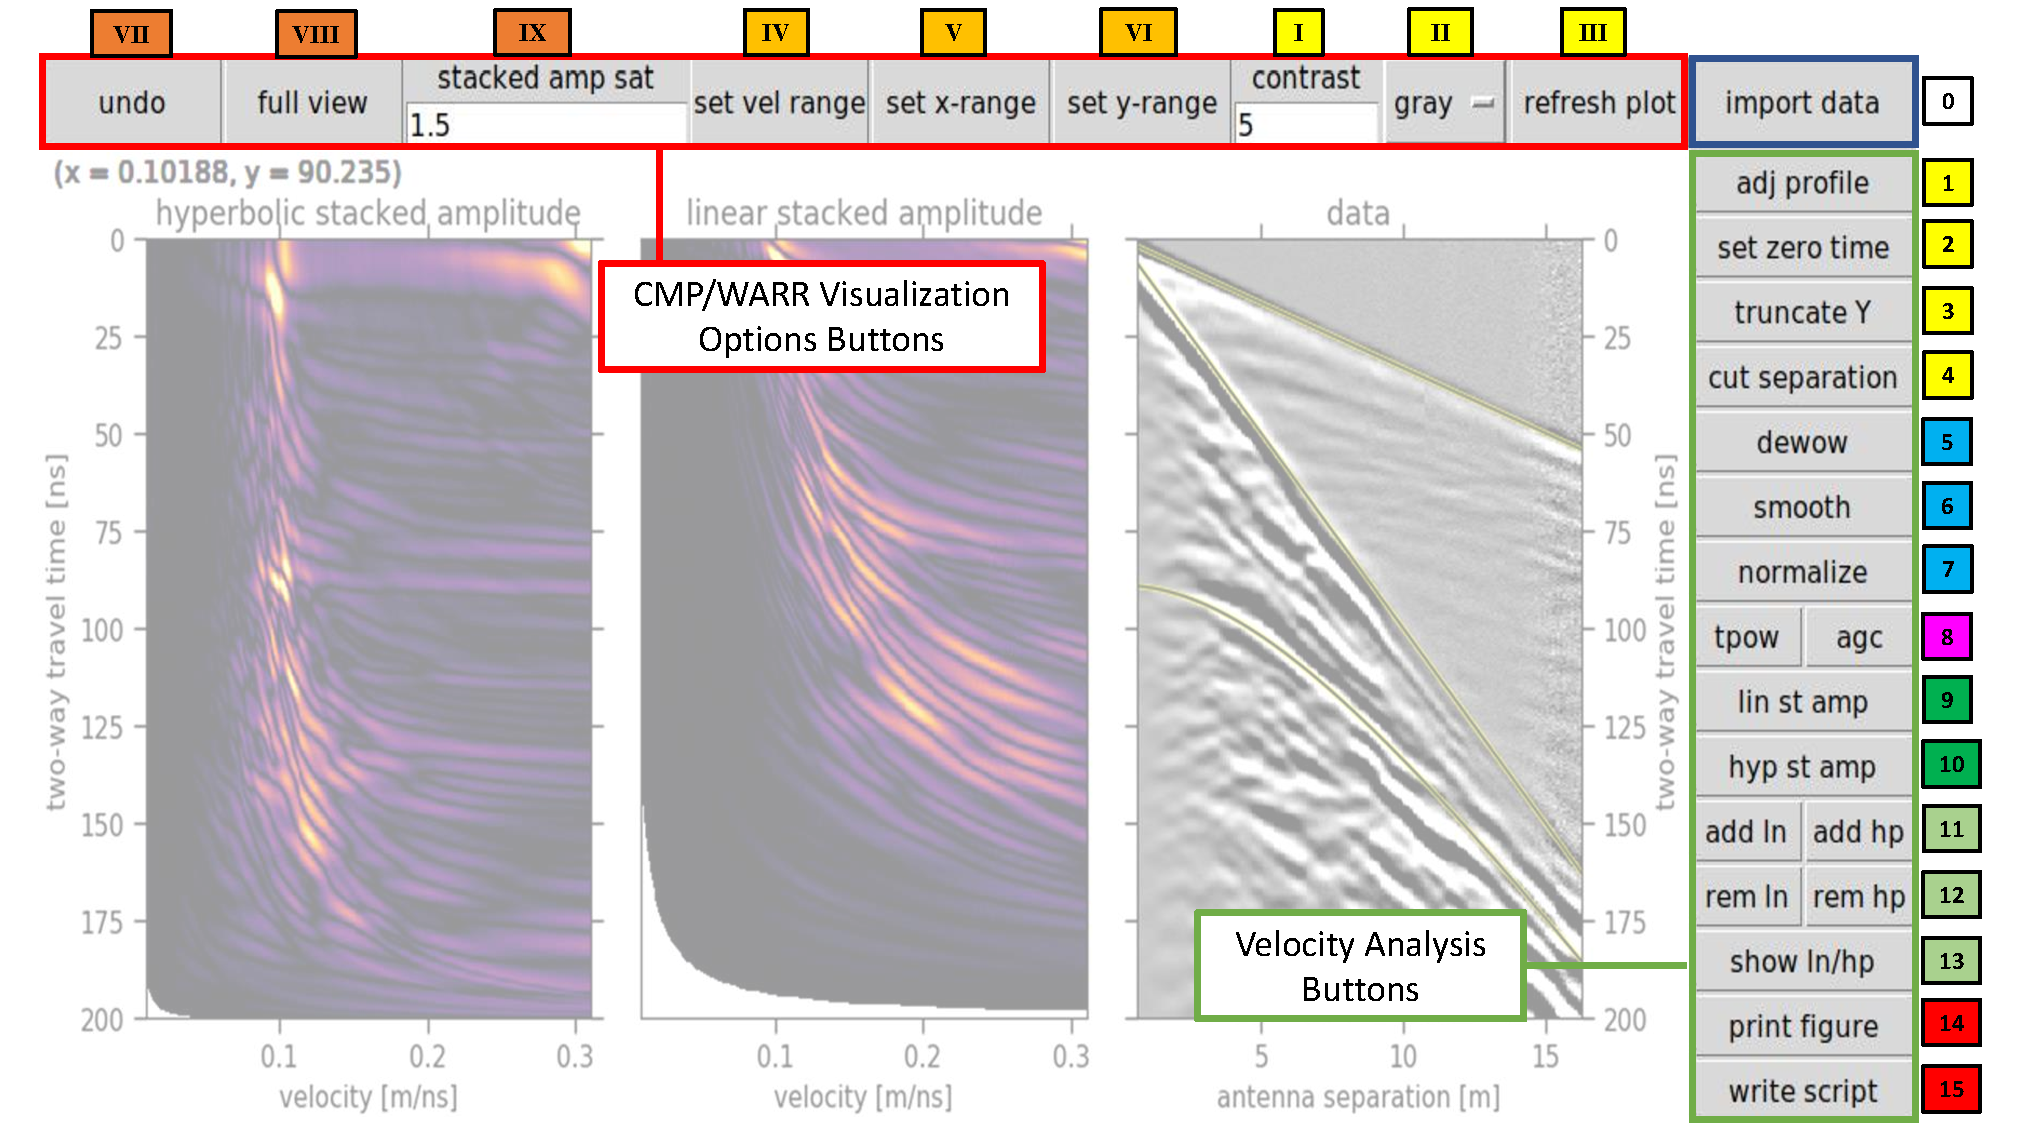
\includegraphics[width=\textwidth]{Figures/Figure2.pdf}
		\caption{GPRPy graphical user interface for CMP / WARR.}

											\end{figure}

First, import your CMP or WARR data by clicking in the option 0, then you should select if your data is a CMP or WARR data.

	\subsection{Cursor Feature – (x,y) Position}
	
	After loading your data, click on any point inside the radar data. A (x,y) coordinate equivalent to the position that you clicked will appear at the top left of the screen (x= distance along the profile and y=two-way travel time). 
	

	\subsection{CMP/WARR Visualization Options Buttons }
	
	Now we can use the following options to facilitate the CMP/WARR visualization: 

\begin{enumerate}[label=\Roman*.]

    \item contrast - Set color saturation.  Click on option Refresh Plot after (\#III).

    \item color scale - Change the color scale been displayed (you can choose gray-scale or red-white-blue (RWB) Click on option Refresh plot after (\#III).

    \item refresh plot -This will allow you to visualize the changes selected in options: \#I, \#II, and \#IX.
    
    \item set x-range - Set the x-axis of the data displays limit. Input a starting point and an ending point.

    \item set y-range - Set the y-axis of the data displays limit. Input a starting point and an ending point.
 
    \item set velocity range - Set the velocity range used in the semblance analysis (\#9 and \#10)
 
    \item undo - Undo your last processing action (only). 
ATTENTION: the option undo, will only undo your last processing action. Clicking on undo multiple times will not bring you to a previous state besides the state of your very last action.  
Example: First you applied Dewow, then you applied AGC, then you decide to undo your processing actions. In this case, clicking on undo, will undo only the AGC, but not the Dewow, even if you click on it twice. 

    \item full view - Allows you to visualize the full profile (resetting the original x-axis and y-axis).

    \item Stacked amp sat - Set the color saturation of the stacked amplitude. 

\end{enumerate}
				
				
						
	\subsection{Velocity Analysis Buttons}
	
	The following table contains the velocity analysis processing buttons and their description. Note that they organized here in the same sequence that they appear in GPRPy (Top-Bottom). 
	
\begin{itemize}
    \item adjust profile - Adjust profile length to a known start and end position. Or flip the profile horizontally (left to right). 
    
Hint: knowing the exactly position of your standing antenna and the final position of the moving antenna is extremely important for a good velocity analysis. Therefore, make sure to check if the antenna separation (x-axis) matches with your minimum and maximum antenna separation. 
    
    \item set zero time - Set the two-way travel time that corresponds to the surface.
To better visualize where to pick the zero time, zoom in the y-axis using the set y-range button (#V). 
You can then click on Full View (#VIII) to restore the visualization or click on the set y-range button (#V) to restore your desired y-range.

    \item truncate y - Remove data points at times latter than the chosen value. If a velocity is given, remove data points deeper than the chosen value.

\item Example: let’s us say that you set the GPR to record all the way to 1000 ns of two-way travel time. But latter you realize that you have interesting data just until 500 ns. You can then click on Truncate Y, and input 500. This will remove every data point beyond 500 ns.

    \item cut separator - Trims data to desired antenna separation range.
Step by Step:
\begin{itemize}
    \item Click on Cut Separator
    \item Input the minimum antenna separation (e.g., 1)
    \item Input the maximum antenna separation (e.g., 24)
\end{itemize}

    \item dewow - Removes from each trace a running mean of the chosen window width (trace-wise low-cut filter). 

    \item smooth - Replace each sample within a trace by a running mean of the chosen window width (trace-wise high-cut filter).
  
    \item normalize - Normalize each trace such that they all have the same energy. 

    \item tpow/agc - These are gain functions. 
     T-power gain: increase the power of the signal by a factor of (two-way travel time) p
     
Automatic Gain Control: Normalize the power of the signal per given sample window along each trace.


    \item lin st amp - Calculate the linear staked amplitude for the selected velocity range (\#VI) and two-way travel times.
Hint:
\begin{itemize}
    \item If the staked amplitude resolution (pixels) is not Satisfactory, you can go back to set vel range (\#IV) and try a smaller velocity step size (interval) (e.g., 0.001). 
    \item Play with the stacked amplitude saturation (\#IX) might also be helpful to visualize the data.
\end{itemize}
 
    \item hyp st amp - Calculate the hyperbolic staked amplitude for the selected velocity range (\#VI) and two-way travel times.
Hint:
\begin{itemize}
    \item If the staked amplitude resolution (pixels) are not good, you can go back to set vel range (\#IV) and try a smaller velocity step size (interval) (e.g., 0.001). 
    \item 	Play with the stacked amplitude saturation (\#IX) might also be helpful to visualize the data.
\end{itemize}

    \item add ln/add hp - Draw line/hyperbola with chosen velocity and intercept two-way travel time on top of data.
Step by Step:
\begin{enumerate}
    \item Click on the position of the line/hyperbola
    \item Click on add ln/add hp
    \item Input a velocity
    \item Input a two-way travel time (y-axis).
\end{enumerate}
  
    \item rem ln/rem hp - Remove the most recent drawn line/hyperbola. 
Hint: you can click multiple times to remove a sequence of added lines our hyperbolas. 

    \item Show ln/hp -  Toggle on/off showing the drawn lines/hyperbolas 

    \item Print Figure - Save the current visible figure with chosen resolution. 
Step by Step:
\begin{enumerate}
    \item Click print figure 
    \item Select where you would like to save it
    \item Select the resolution of the figure (dots per inch).
\end{enumerate}

    \item Write Script - Write a python script to reproduce the current status. 
Note:  If the current data is from .gpr file, then it will contain all the steps going back to the raw data. 
The script will not contain visualization settings such as x and y-rang”, “contrast”, etc. 

\end{itemize}



\section{Automatic Script Generation}\label{Automatic Script Generation}

To run automatically generated scripts, open the command prompt that can run python (for example Anaconda Prompt), switch to the folder with the automatically generated script and run
python myscriptname.py
where myscriptname.py is the name of your automatically generated script.



\section{Three Dimensional Data}\label{Introduction}

When information about the three-dimensional position of a condom-offset profile is available, you can use GPRPy to export that profile as a VTK file, which can be visualized using for example ParaView (Ayachit, 2015).
	In case of a densely spaced and/or interesting profiles are available, then you can use GPRPy to create a three-dimensional cube using the function makeDataCube. This function interpolates the provided profiles and export the resulting data as a VTK file. 



	\subsection{Interpolated Picked Reflectors}
	
	In case three-dimensional interpolation is not possible, due to the lack of data density, but a three-dimensional visualization of specific reflectors can still produce meaningful information, you can use the following steps to create such surface from your GPR data:

\begin{enumerate}
\item Open the graphical user interface for GPRPy Profile.
\item Process your data applying all necessary reductions and corrections. 
\item Find the reflector/structure of your interest. 
\item Click on the button start pick (\#15) on the right side of the interface. \item	Click along the reflector/structure of your interest (a line will start being drawn as you click)
\item Once you are done picking/tracking your reflector/structure, click on stop pick (\#15) on the right side of the interface. 
\item Two files will be created on the folder that your data is located. The first is a x,y file and the second is a x,y,z file (the second one will be created only if you used x,y,z for your topographic correction data.
\item Repeat this process tracking a reflector/structure of interest in other profile(s).
\item Merge together the text files with the information from your tracked reflectors/structures, by copying and pasting the information in a single text file. This is going to be your input.
\item In a separated text file, write the following:

from gprpy.interpSurface import *
interpSurface('input.txt','output',nxgrid=1000,nygrid=1000,method='spline',kx=3,ky=3) 

Change the names “input” and “output” to your files, also change the interpolating options accordingly to your preference and save it. More details about it in Figure 3. You can also simply type the second line on you Python/Anaconda prompt.

												FIGURE HERE!
												
\item Open a Python or Anaconda prompt.
\item In the command prompt, change to the directory where you have your input text file and the text file with the Function call! 
\item Type interpSurface and hit enter.
\item You should now have a vtk file in the same folder with your interpolated surface.
	
\end{enumerate}
	
	\subsection{Data Cube Interpolation}
	
	If there is enough data densely argued (profiles) you can use the function makeDataCube to interpolate your profiles in a data cube following those steps:


1)
2)
3)
4)
5)

from gprpy.makeDataCube import *

 makeDataCube(datalist,outname,nx=50,ny=50,nz=50,smooth=None,nprofile=None,ndepth=None,method='nearest',absvals=False):

												FIGURE HERE!

\end{document}